\section{Stabilität - Nyquistkriterium}{126}
\label{offener Regelkreis}

Die Stabilität eines Regelkreises kann mit dem Nyquistkriterium viel einfacher betrachtet werden. Dafür wird der \textbf{Frequenzgang}
$\boldsymbol{G_0(j \omega)}$ \textbf{des offenen Regelkreises} betrachtet. \\
Ausserdem gibt das Nyquistkriterium an, wie robust ein Regelkreis ist. \\

\begin{minipage}[c]{0.48\columnwidth}
    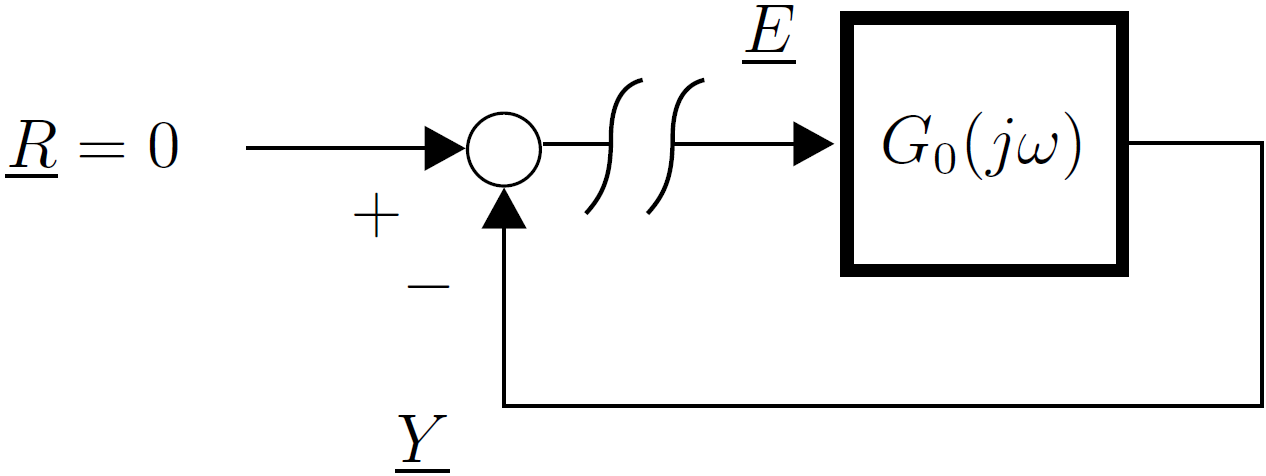
\includegraphics[width=\columnwidth]{images/offener_regelkreis.png}
\end{minipage}
\hfill
\begin{minipage}[c]{0.48\columnwidth}
    \begin{center}
        Frequenzgang des offenen Regelkreises
    \end{center}
    $$ \boxed{ G_0(j \omega) = \frac{\underline{Y}}{\underline{E}} } $$
\end{minipage}



\example{Kreisschaltung mit mehreren Blöcken}
\label{Kreisschaltung mehrere Bloecke}

Folgendes System besitzt ein Eingangssignal $\underline{R}$ und vier Ausgangssignale $\underline{Y}$\\
Es sollen der Frequenzgang des offenen Regelkreises $G_0(j \omega)$, sowie ausgewählte UTFs des Systems beschrieben werden.

$$ G_0(j \omega) = G_1(j \omega) \cdot G_2(j \omega) \cdot G_3(j \omega)  $$

\begin{minipage}[c]{0.5\columnwidth}
    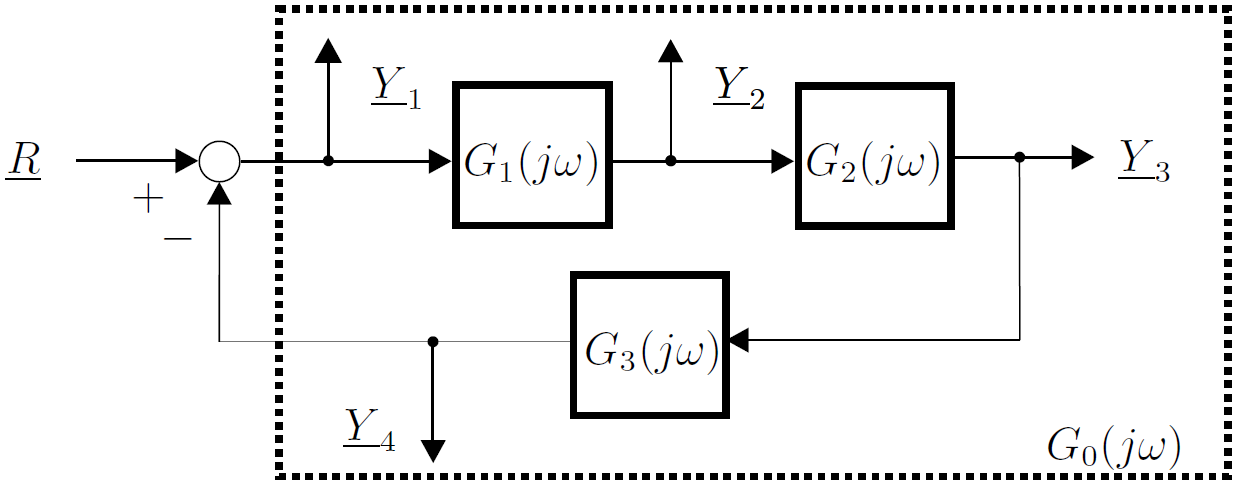
\includegraphics[width=\columnwidth]{images/kreisschaltung_mehrere_bloecke.png}
\end{minipage}
\hfill
\begin{minipage}[c]{0.48\columnwidth}
    $$ \frac{\underline{Y}_1}{\underline{R}} = \frac{1}{1 + G_1(j \omega) \cdot G_2(j \omega) \cdot G_3(j \omega)} $$
    % $$ \frac{\underline{Y}_1}{\underline{R}} = \frac{G_1(j \omega)}{1 + G_1(j \omega) \cdot G_2(j \omega) \cdot G_3(j \omega)} $$
    $$ \frac{\underline{Y}_3}{\underline{R}} = \frac{G_1(j \omega) \cdot G_2(j \omega)}{1 + G_1(j \omega) \cdot G_2(j \omega) \cdot G_3(j \omega)} $$
    % $$ \frac{\underline{Y}_4}{\underline{R}} = \frac{G_1(j \omega) \cdot G_2(j \omega) \cdot G_3(j \omega)}{1 + G_1(j \omega) \cdot G_2(j \omega) \cdot G_3(j \omega)} $$
    
\end{minipage}


\subsection{Stabilität im Nyquist-Diagramm}

Gedankenexperiment: Ein offener Regelkreis mit $G_0(j \omega)$ (gemäss Abschnitt ~\ref{offener Regelkreis}) um eine 
veränderbare Verstärkung $K$ ergänzt.


\subsubsection{Stabilität}

Wähle $K = K_0$, sodass sich die Ortskurve immer innerhalb des Einheitskreises befindet.
\vspace{0.1cm}
\begin{itemize}
    \item Befindet sich die Ortskurve eines Systems immer \textbf{innerhalb des Einheitskreises}, so ist der offene Regelkreis stabil. \\
        \textrightarrow Daraus folgt, dass auch der geschlossene Regelkreis stabil sein muss.
    \item Führungsübertragungsfunktion für $K \ll K_0$:\\
    $G_f(j \omega) = \frac{K \cdot G_0(j \omega)}{1 + K \cdot G_0(j \omega)} \approx K \cdot G_0(j \omega)$ 
\end{itemize}


\subsubsection{Grenzstabilität}

Wähle $K = K_{krit} > K_0$, sodass die Ortskurve den Punkt $-1$ schneidet.
\vspace{0.1cm}
\begin{itemize}
    \item Ortskurve des offenen Regelkreises $G_0(j \omega)$ verläuft \textbf{durch den Punkt $\boldsymbol{-1}$}, 
    \item Die Frequenz $\omega_{\pi}$, für die $G_0(j \omega_{\pi})= -1 = e^{- \pi}$ heisst \textbf{kritische Frequenz}. Mit dieser 
        kritischen Frequenz schwingt das System.
    \item Die Führungsübertragungsfunktion $G_f(j \omega) = \frac { K \cdot G_0(j \omega)}{1 + K \cdot G_0(j \omega)}$ wird bei 
    der kritischen Frequenz zu $G_f(j \omega_{\pi}) = \frac{-1}{1-1} = - \infty $ \textrightarrow Grenzstabilität
\end{itemize}


\subsubsection{Instabilität}

Wähle $K > K_{krit}$
\vspace{0.1cm}
\begin{itemize}
    \item Ortskurve verläuft nicht mehr durch den Punkt $-1$
    \item Das System ist instabil
\end{itemize}


\subsection{Vereinfachtes Nyquistkriterium}{127-128}

Idee: Informationen über den \textbf{offenen Regelkreis} verwenden, um die \textbf{Stabillität des geschlossenen Regelkreises} 
zu beurteilen



\subsubsection{Vereinfachtes Nyquistkriterium}

\fbox{\parbox{0.95\columnwidth}{
\begin{itemize}
    \item Gemäss Abschnitt ~\ref{Kreisschaltung mehrere Bloecke}  wird $G_0 = \prod_i G_i$ gebildet aus den seriegeschalteten
        Teilsystemen des offenen Regelkreises
    \item $G_0$ muss dabei einem \textbf{Prozess mit Ausgleich} entsprechen; zusätzlich \textbf{dürfen} noch einer oder zwei 
        Integratoren seriegeschaltet sein\\
        Mit Polen formuliert: Bei $G_0$ sind maximal zwei Pole bei Null erlaubt; alle weiteren Pole müssen in der linken Halbebene liegen
    \item Damit der geschlossene Regelkreis stabil ist, muss der kritische Punkt $-1$ \textbf{links} der Nyquistkurve von $G_0$ liegen,
        wenn diese in Richtung zunehmender Frequenz durchlaufen wird ($\omega = 0 \ldots \infty$)
\end{itemize}
}}


\example{Ortskurven stabiler Systeme}{128}

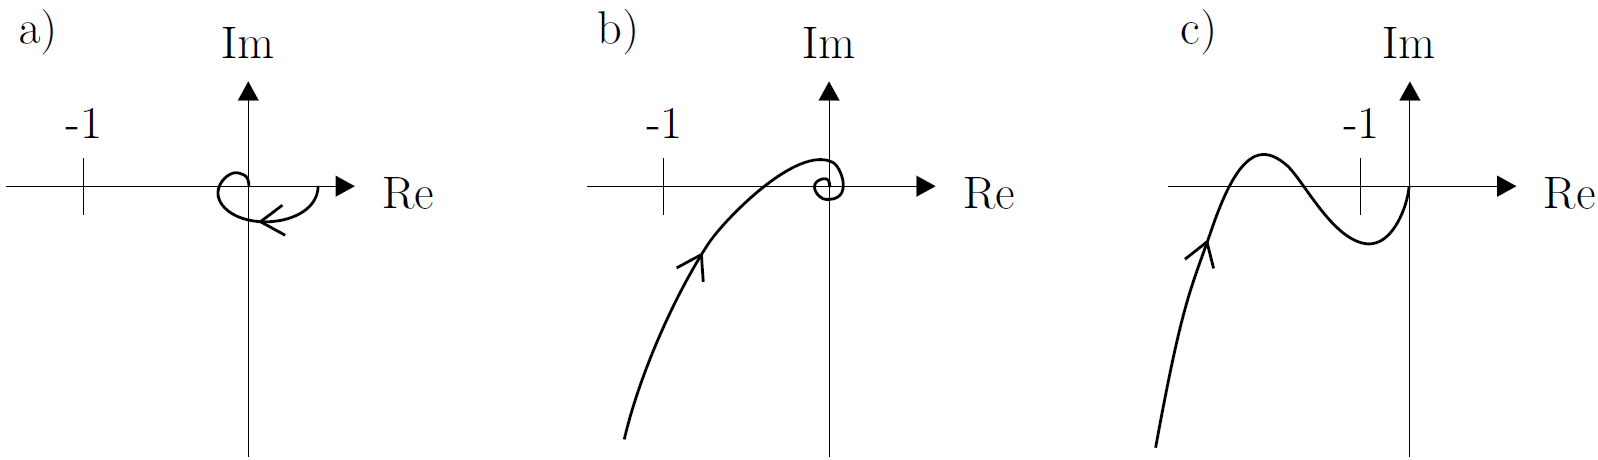
\includegraphics[width=\columnwidth]{images/nyquist_stabile_kurven.png}
